\documentclass[conference]{IEEEtran}
\IEEEoverridecommandlockouts


\usepackage[pdftex]{graphicx}
\usepackage{amsmath,amssymb,amsfonts}
\usepackage{algorithmic}
\usepackage{graphicx}
\usepackage{float}
\usepackage{comment}
\usepackage{movie15}
\usepackage{textcomp}
\usepackage{xcolor}
\usepackage[style=ieee]{biblatex}
\addbibresource{paper.bib}
\usepackage{url}
\usepackage[linkcolor = blue]{hyperref}
\newcommand{\MYhref}[3][blue]{\href{#2}{\color{#1}{#3}}}

% correct bad hyphenation here
\hyphenation{op-tical net-works semi-conduc-tor}

\newcommand{\todo}[1]{{\color{olive} TODO: #1}}

% Regler til skrivning: 
% 1. Altid nutid
% 2. Brug 1. persons flertal stedord (We/us/our/ours)
% 3. Skriv formelt og uden sammentrækninger (don't do this) 
% 

\begin{document}

\title{Telemetry Module for Solar Vehicle}

\author{\IEEEauthorblockN{Victor Alexander Hansen s194027, Steffan Martin Kunoy s194006, Tjark Petersen, s186083}
\IEEEauthorblockA{\textit{Department of Electrical Engineering} \\
\textit{Technical Uniservity of Denmark}\\
Kgs. Lyngby, Denmark \\
31015 Introductory project - electrotechnology\\
s194027@student.dtu.dk, s194006@student.dtu.dk, s186083@student.dtu.dk}}
%\author{Victor Alexander Hansen, Steffan Martin Kunoy, Tjark Petersen}

\maketitle

% As a general rule, do not put math, special symbols or citations
% in the abstract or keywords.
\begin{abstract}
This paper presents the telemetry project for the DTU ROAST Solar car. The development of the module is done through design sprints, where hardware and software is gradually developed along side each other. First a Hardware prototype on breadboards, then the software to run the modules satisfactorily was developed and finally the final product was made when the hardware was soldered to perf boards.\\
The software developed for the module provided the module to have two-way communication with CAN message structure, encryption of the data during transmission between the module in the solar car and a module in a support car, the ability to give the solar car module commands from the support car and streaming received messages in the support car to Matlab.
\end{abstract}

% Note that keywords are not normally used for peerreview papers.
\begin{IEEEkeywords}
ROAST, telemetry, CAN, RSA encryption, Matlab
\end{IEEEkeywords}



\section{Introduction}

\IEEEPARstart{I}{n} 2023, the DTU Roadrunners Solar Team (abbreviated ROAST) is set to participate in the Bridgestone World Solar Challenge, a race spanning over 3000 km across Australia from Darwin in the Northern Territory to Adelaide in South Australia. The solar car has limited opportunities for recharging during the race, so its the main energy source will be the sun. To this end, solar panels will cover the car, however, the solar car is only allowed to have a maximum of 4 square meters of solar panels. This emphasizes the need to create an energy-efficient solar car to win the race \cite{wsc}.

Throughout the race the solar car will be monitored by a support vehicle, which can monitor the car's condition and should be able to issue commands to the solar cars internal systems. This is a crucial function as the solar car will be navigating Australia's busy highways, where the heat and tire pressure may cause a detriment to the vehicle. The support vehicle will therefore be able to analyze and react to the data stream being transmitted from the solar car, even when the driver is preoccupied with driving the car. 

Additionally, valuable data can be collected during the race which can help to identify possible areas of improvement of the solar car. Therefore a "black box" system is needed to capture all system activity in a local storage.

These key functionalities require a system which is able to read and write data from the solar cars on-board CAN (Controller Area Network) bus and transmit it via an RF-transceiver to the support vehicle, while simultaneously logging data locally. The support vehicle is equipped with a similar module such that the support crew can react to the data manually or automatically by sending commands back to the CAN bus via RF. Thus, the capabilities of such a telemetry module play a vital role in the communication between both vehicles, considering that the distance between them may be up to 1 km depending on traffic conditions.

\begin{figure}[b]
    \centering
    
\includegraphics[width=0.5\textwidth]{documentation/images/SolarChallengeLogo.pdf}
    \caption{Bridgestone World Solar Challenge logo \cite{wsc}.}
    \label{fig:solar}
\end{figure}

The telemetry system must both serve the purpose of fulfilling the necessary specifications for communication, while also being as energy-efficient as possible. This project aims at implementing a functioning prototype for a telemetry system while mainly focusing on the former of the two objectives, that is, ensuring that the system meets the specifications with a solid solution.

This paper begins with giving a more precise problem statement and introducing the methodology used throughout the project. Thereafter, the overall system design is presented and the following paragraphs discuss the hardware components and software used for these. After this comes a paragraph discussing the implementation of the communication between the two modules, both internal and during transmission. This concludes with a section of the final product, which is followed up by our method method for testing and validating our solution, as well as discussion and conclusion of the solution.

\subsection{Problem Statement}
Remote sensing of data from the solar car will give the ROAST team a competitive advantage as the support vehicle will be able to take on a more active role in managing and optimising the car's performance. This will ease the burden on the driver and leverage the expertise of the supporting crew. For these reasons we have chosen to focus our project on the following points:
\begin{itemize}
    \item How can we design a module that can read and write sensor data and commands from a CAN bus network? 
    \item How can CAN data be transmitted securely over a distance of up to one kilometer?
    \item How does the support-car module process data upon receiving it from the solar car?
    \item What is the best method for storing data locally (black box) while being accessible at a later time?
    \item How can the CAN data be made accessible in the support vehicle for further processing e.g. in Matlab?
\end{itemize}

\section{Methodology}
The project methodology has largely consisted of making a preliminary design to be completed in a series of design sprints. At first a detailed specification was drafted which then served as a reevaluation tool and an overall guidance each time a sprint was completed and when the goal for the next sprint had to be selected. Using the specification, we made a prototype setup of the hardware on breadboards as our first sprint. The following sprints would then mostly have software development objectives, such as achieving a first transmission and receiving of data. Finally, a last hardware sprint was conducted where we soldered our hardware to a perf board.

During the development of the software functions, we also verified and validated our code design. In verification the code and its functionality was discussed. To validate our code we made unit tests that test the actual behaviour of our code against the intended behaviour.

During the software development phase, we attempted to make our debugging more efficient with the use of a debugger. However, this proved quite troublesome, as the Teensy 3.6 board does not have an on-board debugger and in general is not very suited for debuggers. If we had insisted on using a debugger such as st-link, we would have had to hold or solder wires to the debug ports on the Teensy board's backside, which would complicate our prototype setup. Therefore, we decided not to spent more time on finding a debugger solution. This was a clear setback, as debugging could only be conducted by sending text over the serial connection.

\section{Design}
The overall system consists of three separate modules; the Solar Car Unit (SCU) which is connected to the CAN bus and communicates with the support vehicle unit via a wireless RF connection. The Support Vehicle Unit (SVU) in turn interacts with the Support Vehicle laptop through a serial connection. The GUI program running on the laptop broadcasts the CAN bus message stream on the local network. A block diagram for the system is outlined in Fig. \ref{fig:schematic}. 
\begin{figure}[H]
    \centering
    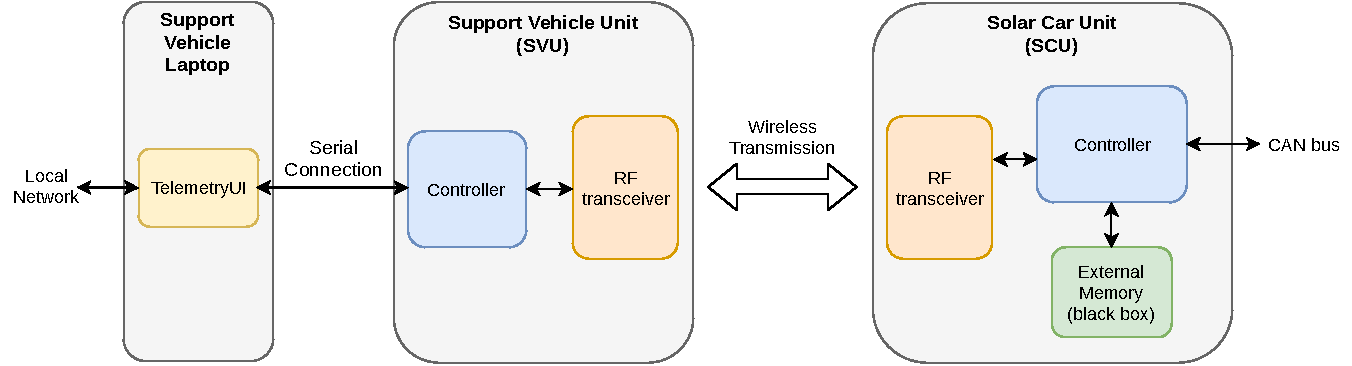
\includegraphics[width=0.5\textwidth]{documentation/images/SystemSchematic.pdf}
    \caption{Overview of the system's components in block diagram form.}
    \label{fig:schematic}
\end{figure}


\section{Components}

\subsection{Microcontrollers} % Steffan
We use Teensy 3.6 and 4.0 microcontrollers as connection hubs in the SCU and SVU, respectively. The Teensy line-up has been used as the main microcontroller platform in most ecocar projects and we decided to use them as well after considering the performance of newer Teensy boards. The boards can interact with the various components through an SPI interface to gather, process and transmit large amounts of data. Being based on the Arduino framework, both Teensys offer support for numerous protocols and software libraries to ease the implementation of our design. 

\subsection{CAN bus}
The CAN network in the SCU enables all the car's processing nodes to send and receive data without a host computer. This is possible thanks to the special structure of the CAN message.

\begin{figure}[h]
    \centering
    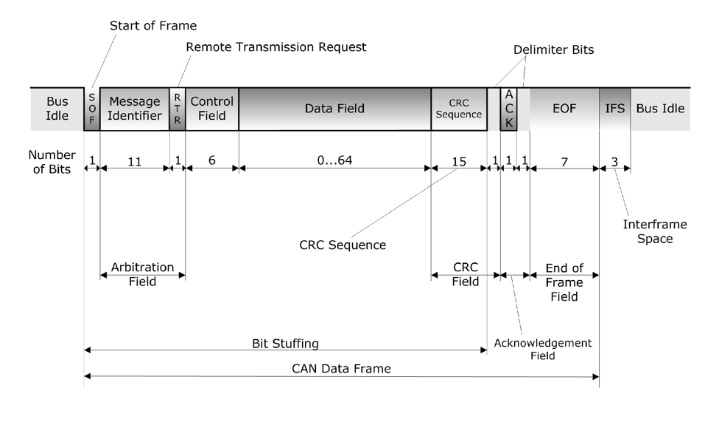
\includegraphics[scale=0.35]{documentation/images/detailed-can-data-frame-architecture.jpg}
    \caption{Structure of a CAN frame.}
    \label{fig:CANframe}
\end{figure}

The frame uses an identifier to tell which messages goes to which unit. When two messages try to access the bus, the one with the highest priority (lowest ID) will be granted access to the bus, while the other message have to wait. After the ID comes the RTR bit which determines whether the frame remotely requests or actually sends data to a node. The control field, sometimes called DLC, holds the amount of bytes used in the following frame field containing the actual data. The rest of the fields in fig. \ref{fig:CANframe} serve error checking and coordination of communication on the bus.

The physical CAN bus itself consists of a differential pair of twisted wires, CAN High and CAN Low. These control the bits in the CAN message by setting a dominant and recessive voltage, which corresponds to a 0 and 1 respectively. A 1 is seen when the voltage in both wires is 2.5V while a 0 is seen when the CAN High wire is driven by 3.75V and the CAN Low wire is driven at 1.25V. 

The Teensy 3.6 used in the solar car features a CAN controller handling message assembly and receiving from the CAN bus. In order to interface with the physical CAN bus though, a transceiver is needed. Here the MCP2551 was chosen since it has been used extensively in other ecocar projects. The component maintains one input and one output serial stream to the CAN controller on the Teensy and drives the CAN bus when a message is transmitted.

\subsection{RF network} % Steffan
Two radio-frequency (RF) transceivers are required to provide a stable connection between the SCU and SVU at longer distances. There are many options for radio modules supporting long range communication at the expense of achievable data rate. We chose a trade-off between both by selecting the nRF24L01+ operating on the 2.4 GHz ISM band. The module features a detachable antenna, power amplifier and low-noise amplifier to provide a theoretical range in excess of 1000 m and data transfer rates of up to 2 Mbit/s.

An advantage of using the off-the-shelf RF module is the automated message protocol, known as Enhanced Shockburst$^\copyright$ \cite{shockburst}. Messages are transmitted in packages, structured in flexible byte segments, as shown in Fig. \ref{fig:shockburst}. Only the data payload and address needs to be specified prior to sending a package; the preamble, packet and CRC segments are generated automatically and therefore fall beyond the scope of this project. 

\begin{figure}[h]
    \centering
    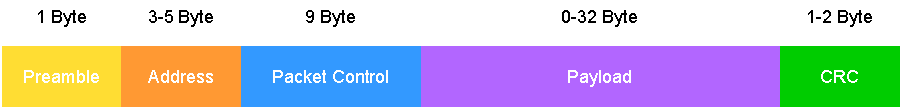
\includegraphics[width=0.5\textwidth]{documentation/images/EnhancedShockburst.pdf}
    \caption{The Enhanced Shockburst$^\copyright$ packet structure.}
    \label{fig:shockburst}
\end{figure}

\subsection{SD card}

We chose a SD card as a permanent local storage solution for the SCU's "black box" due to its ease of use and accesibility through the Teensy 3.6 integrated SD card slot. Furthermore, this solution scales very well and easily in terms storage capacity, with new SD card sizes exceeding 1 TiB.

\section{Software Stack}

Several of the key functionalities of the telemetry module are implemented in software. This, together with the aim of designing a system to be expanded upon in the future, makes the choice of software frameworks very important. Thus, an emphasis has been placed on the reusability and maintainability of the developed code.

\subsection{Build system}
As a build system, PlatformIO \cite{platformIO} was chosen for the project. It is a version control friendly, cross-platform embedded build tool which includes library management and works by defining \textit{environments} to allow development with different embedded platforms on the same code base. It comes with a VScode plugin for ideal IDE support. Other project groups working on the solar car in parallel integrated their software into the PlatformIO ecosystem as well, making extensive code reuse in the future possible.

\subsection{Real Time Operating System}
We chose to build the software for the telemetry system on top of a real time operating system. The small kernel running behind the scenes when using a RTOS allows a step up in abstraction from bare metal programming. Different tasks can be spawned as threads running concurrently. These threads get delegated time slices to run on the processor by the real time kernel based on their priority. 

This comes at the cost of introducing overhead when switching between threads, but the great flexibility in code organization following with an RTOS was evaluated to make the overhead a worthwhile trade-off.

As a specific RTOS, we chose ChibiOS \cite{chibios}, since it is supported on both the Teensy 3.6 and 4.0 and since it attempts to keep the memory footprint of the real time kernel as small as possible.

\subsection{Graphical User Interface} % Tjark

The GUI included in the telemetry system serves a proof-of-concept purpose. Therefore, scala-swing \cite{scala-swing} was chosen as a framework, due to the effectiveness of the scala \cite{scala} language and the high level of abstraction used when describing a user interface in scala-swing. Furthermore, a GUI implementation in scala can run on any system with a java virtual machine and is therefore cross-platform compatible.

In order to send and receive data from the SVU via serial connection, the jSerialComm \cite{jSerialComm} library was used.

\subsection{Data Processing} % Steffan
Due to the wishes of DTU ROAST to use the telemetry data in applications of predictive modelling and performance optimization we decided to implement a simple UDP network stream hosted on the Support Vehicle laptop. This would allow all devices on the local network to monitor the data being sent over the serial connection for use in further data processing. For a proof-of-concept case we created a simple Matlab script to sample CAN messages from the UDP port and print them formatted to the terminal. 

\subsection{Other Libraries}
In order to interface with the components presented in the previous section, a set of libraries were included in the project. These include a CAN network driver to support use of the Teensy 3.6's integrated CAN controller \cite{ACAN}, an RF OSI layer providing seamless integration with the nRF24L01+ modules, and an SD card driver to control data logging in the black box memory. 

%In order to interface with the components presented in the previous section, a set of libraries were used.

%The ACAN library by Pierre Molinaro is a CAN network driver for the Teensy 3.6 board, as well as older Teensy series 3 boards. The library has been important for the connection between the CAN network and the ports on the Teensy board. We have only used the classic CAN configuration, but in addition to this, the library supports Flex CAN and CANFD. The driver supports bit rates ranging from 62.5 kbit/s up to 1 Mbit/s.

\section{Internal Communication}
The main function of the telemetry system is to bridge data streams between different end points. As such, a flexible way to pass commands and associated data payloads both ways through the system is needed. 

The majority of messages passed between the two telemetry subsystems will contain CAN messages as part of the stream from the solar car to the support vehicle. Therefore, the message protocol is designed around 16 byte messages, which are large enough to comfortably fit a CAN message and a time stamp from when the message was received. A diagram of the byte layout of a message is shown in figure \ref{fig:messageTypes}.

\begin{figure}
    \centering
    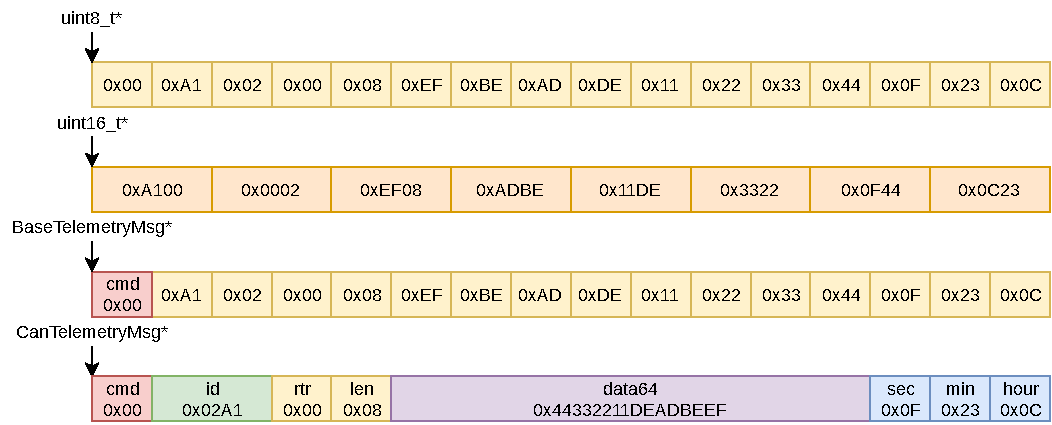
\includegraphics[width=\linewidth]{documentation/images/MessageTypes.pdf}
    \caption{The different message types used in the telemetry system.}
    \label{fig:messageTypes}
\end{figure}

The system is built around \textit{commands} and \textit{message types}. All message types begin with a command byte. The remaining 15 bytes are interpreted based on the message type. As an example, a \texttt{CanTelemetryMsg} message type is shown in figure \ref{fig:messageTypes}. 

One message type can be connected to different commands. For instance, the \texttt{CanTelemetryMsg} message type can be used to send data from the SCU to the SVU as part of the data stream setting the command to \texttt{RECEIVED\_CAN} = \texttt{0x00} or it can be used to inject a CAN message from the SVU into the solar car's CAN bus setting the command to \texttt{BROADCAST\_CAN} = \texttt{0x01}. 

When decoding messages, only the first byte needs to be considered and it will unambiguously decide how the rest of the message should be interpreted. This eases the decoding of messages on the receiving end and makes for a expandable framework which has enough room for future expansions. 

Even though some message types are only sent one direction between the telemetry modules, a unified design was chosen due to the inherent simplicity.

As an extra feature not included in our original specification, we have made an encryption protocol for our telemetry module. The encryption is based on the RSA algorithm, which essentially generates an encryption key based on the modulus and totient function of two prime numbers. The pairings of prime numbers suited for the encryption protocol can be seen in Fig. \ref{fig:prime_tabel}. 

When a message is encrypted, each of the 16 bytes is extended to a 16-bit unsigned integer to avoid overflow problems increasing the total message size to 32 bytes. Once transmitted to the receiving node, the message is then decrypted and the overflow protection bytes can be removed leaving us with 16 bytes again. This essentially doubles the size of the data payloads being sent in our RF transmission, which is the downside of our encryption solution.

\begin{figure}
    \centering
    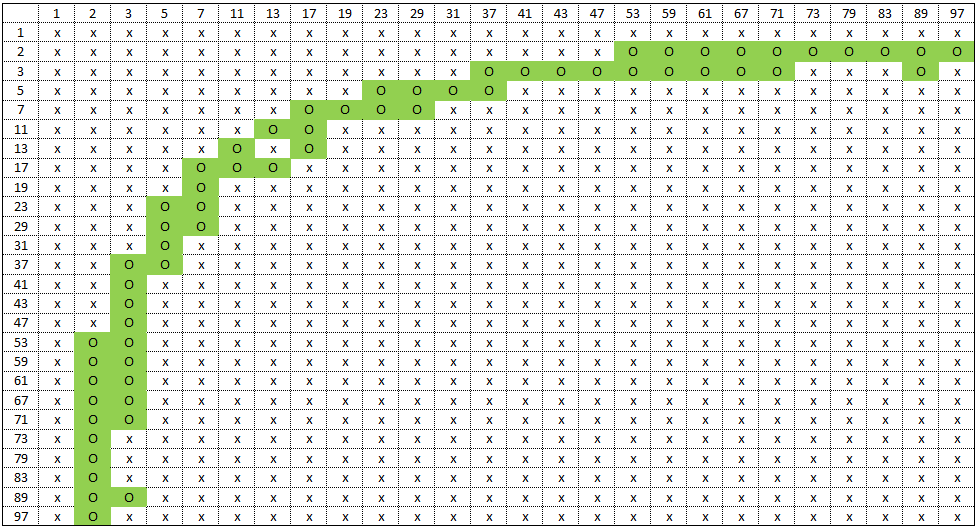
\includegraphics[width=\linewidth]{documentation/images/prime_tabel.png}
    \caption{Valid combinations of prime numbers, marked by O}
    \label{fig:prime_tabel}
\end{figure}


\section{\todo{Final product}}
\subsection{Solar Car Unit}

% actual circuit
% - powered through molex connector 12V
% - converted to 5V and teensy internal voltage regulator to 3.3
% - Teensy has RTC which can keep time when powered by an external 2.9V battery

% on the software side
% - threads:
%  - 

\begin{figure}
    \centering
    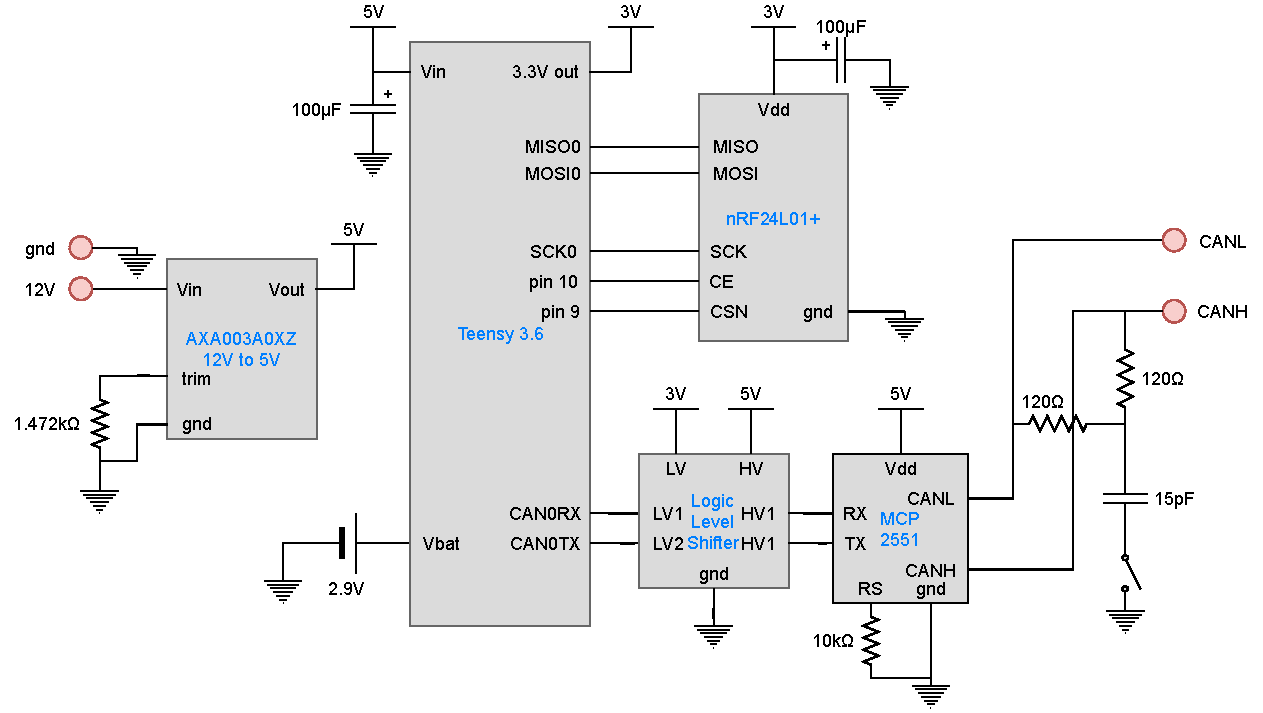
\includegraphics[width=\linewidth]{documentation/images/SCU_CircuitDiagram.pdf}
    \caption{The circuit diagram for the SCU.}
    \label{fig:SCU_circuit}
\end{figure}
% threads 
\subsection{Support Vehicle Unit}
\begin{figure}
    \centering
    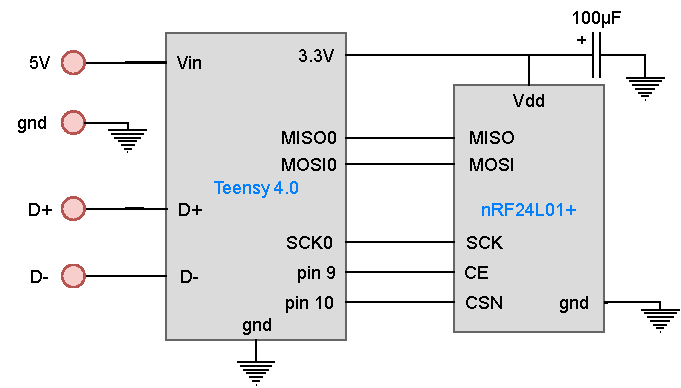
\includegraphics[width=\linewidth]{documentation/images/SVU_CircuitDiagram.pdf}
    \caption{The circuit diagram for the SVU.}
    \label{fig:SCU_circuit}
\end{figure}
% threads
\subsection{\todo{Graphical User Interface}}
% GUI 


\section{Verification and Validation} % Victor
As mentioned in the methodology section, we spent time thoroughly verifying and validating our code design. We undertook the software verification after finishing the prototype and software coding, reviewing the naming, functionality and commenting the code accordingly.

We performed software validation concurrently with writing our code to make sure that the actual behaviour of the program matched the expected behaviour. This was done through the testing environment in PlatformIO. We used this to validate our code design with unit tests, testing both edge cases and random cases. We chose only to validate the code and functions we made ourselves, and not those that was imported from external libraries.

Doing this provided us a test bench for our project, which greatly improved the credibility of our work, proving that our design works in general cases and not just the case we represent in our report.

\section{Discussion}

% range test
In order to test the connection between the Solar Car and Support Vehicle modules we performed a range test in a suitable outdoor environment. In the end, we achieved a transmission range of around 160 m before the connection became too unreliable. A video documenting the test can be viewed with \MYhref{https://youtu.be/-iwST3REn40}{this link}. This is obviously a big step down from the 1000 m claimed by the manufacturer. However, considering the crude implementation of our hardware components, as well as the interference from buildings and other vehicles, that range was highly unattainable in the first place. Further enhancements in the hardware, such as a stable power supply for the RF modules, would likely improve the range beyond 400 m. 
 
% throughput limitations
% variable length messages would reduce overhead -> but most messages contain CAN and are optimized
% UDP works only one way for now. If automated control from matlab should be possible, udp listeners should be able to send as well

\section{Conclusion}
%The conclusion goes here.



\section*{Acknowledgment}
The authors would like to thank Martin Schoeberl and Christian Kampp Kruse for their mentoring and assistance throughout the project. The authors would also like to thank Claus Suldrup Nielsen from the department of Mechanical Engineering at DTU.


\printbibliography

\end{document}
